\documentclass{BeamerTemplate}

\usepackage{pgfplotstable}
\pgfplotsset{compat=1.17}

% Données de l'exemple : production (kg) de 60 plants de tomates
\pgfplotstableread{
x y
3 2.92
3 2.59
3 2.73
3 2.43
3 3.78
3 2.23
3 3.07
3 1.69
3 1.98
3 2.95
4 2.54
4 2.92
4 3.65
4 3.57
4 3.60
4 2.41
4 3.79
4 2.74
4 2.41
4 3.49
5 3.17
5 2.72
5 4.53
5 3.21
5 3.00
5 4.15
5 2.99
5 4.48
5 3.17
5 3.82
6 4.13
6 4.64
6 4.55
6 3.42
6 4.23
6 3.76
6 3.57
6 4.94
6 3.93
6 3.46
7 3.42
7 5.20
7 4.63
7 4.16
7 3.64
7 3.61
7 4.44
7 4.46
7 5.08
7 4.23
8 4.08
8 5.43
8 5.76
8 3.99
8 4.55
8 4.93
8 5.11
8 5.00
8 4.86
8 4.72
}\tomates

% Paires de variables normales centrées réduites non corrélées (simulées),
% utilisées pour illustrer différents coefficients de corrélation.
\pgfplotstableread{
z1 z2
2.003 -2.500
0.438 -0.585
-0.403 -0.273
-1.915 -0.362
-0.801 3.250
0.252 -0.379
-0.237 -0.718
-0.984 -0.476
0.499 -0.253
0.958 -0.192
0.057 1.512
0.560 -0.517
-0.142 0.496
1.901 -0.217
-0.201 0.956
-0.821 -0.369
0.886 0.586
0.122 0.639
-2.695 0.855
-0.892 -1.751
0.301 0.678
-0.395 -1.134
0.059 -0.088
1.390 0.777
0.221 1.085
-0.164 -0.972
0.598 0.574
-0.173 -0.830
0.255 -2.522
0.700 0.488
-1.547 -0.051
-0.896 0.677
-1.929 -1.046
0.719 1.154
-2.048 -0.634
0.351 -0.631
1.569 -1.155
0.376 -1.069
1.391 0.007
-0.325 -1.773
1.657 0.795
0.761 1.138
0.371 -0.660
-0.738 -0.874
1.356 -1.435
-0.541 -0.385
0.251 0.550
-1.171 -1.826
0.030 1.178
0.765 0.215
-0.272 0.243
-0.201 0.771
-0.733 0.061
-0.073 0.503
0.251 2.527
1.480 1.531
-1.934 -0.471
-0.553 0.469
-2.165 1.034
1.064 -1.290
-0.910 -0.883
0.076 0.607
2.010 -0.139
0.775 0.155
1.732 0.788
1.355 -1.052
-0.151 -0.860
1.486 0.692
-0.260 -0.503
0.502 -0.716
-0.864 0.403
2.411 -0.169
-0.502 -1.234
-1.254 0.428
0.855 0.012
0.355 0.095
0.168 -1.557
-0.408 0.054
-0.722 -0.549
-0.756 -0.408
0.857 -0.404
-0.114 0.771
0.656 1.690
-1.983 0.725
-0.431 0.076
0.842 1.087
1.037 0.167
1.587 -0.245
-0.102 0.757
-0.498 2.101
1.018 2.189
0.008 -0.421
0.195 0.707
-0.533 0.317
0.018 1.580
-0.605 0.980
-0.587 -1.027
-0.651 -1.260
0.175 1.003
0.193 0.596
1.609 0.310
0.222 -0.302
-1.518 0.650
-1.661 0.536
0.020 1.091
-0.031 -0.863
0.379 -0.580
-0.141 -0.003
-0.096 -0.231
-0.769 -0.264
-2.029 -0.292
-1.122 1.030
1.260 -1.930
0.174 -0.156
-0.976 0.448
-0.411 -1.827
-0.223 -0.197
0.137 -1.264
0.628 0.728
-1.072 -0.749
}\normales

% Droite estimée et quantités utiles (exemple des tomates)
\def\bzero{1.37242}
\def\bun{0.43126}
\def\mse{0.32278}
\def\tq{2.0017}

\pgfplotsset{
  tomates/.style={
    width=9.5cm, height=5.8cm, xmin=2.6, xmax=8.4, ymin=1.4, ymax=6,
    xlabel={Heures d'ensoleillement}, ylabel={Production (kg)},
    tick label style={font=\scriptsize}, label style={font=\small},
    grid=major, grid style={black!10},
  },
  nuage/.style={
    width=4.2cm, height=4.2cm, ticks=none, title style={font=\scriptsize},
    xmin=-3.3, xmax=3.3, ymin=-3.3, ymax=3.3,
  }
}

\title{Chapitre 6b -- Régression linéaire simple (suite)}
\subtitle{STT-1920 Méthodes statistiques}
\date{}

\begin{document}
\begin{frame}[t]
  \titlepage
\end{frame}

\begin{frame}[t]{Plan}
\tableofcontents
\end{frame}

%-------------------------------------------------------------------------------
\section{Prédictions}
%-------------------------------------------------------------------------------

\begin{frame}[t]{Intervalle de confiance pour la moyenne de $Y$ en $x^*$: exemple}

On voudrait construire un intervalle de confiance à 95\,\% pour la
\alert{production moyenne} attendue de \alert{tous} les plants ayant reçu
6,5 heures d'ensoleillement par jour.

\medskip
\small
Rappel des calculs du chapitre 6a: $\overline{x}=5{,}5$, $\overline{y}=3{,}744$,
$S_{XX}=175$, $S_{XY}=75{,}470$, d'où
\[
b_1=\frac{75{,}470}{175}=0{,}4313,\quad b_0=3{,}744-0{,}4313\times5{,}5=1{,}3724,\quad
\hat\sigma^2=MSE=0{,}3228.
\]
La droite de régression estimée est donc $\hat y=1{,}3724+0{,}4313\,x$.

\end{frame}

\begin{frame}[t]{IC pour la moyenne de $Y$ en $x^*$}

La valeur moyenne de $Y$ lorsque $X=x^*$ est le point sur la vraie droite en
$x^*$: $\beta_0+\beta_1x^*$, estimé par $b_0+b_1x^*$. On peut montrer que
\[
b_0+b_1x^*\sim N\left(\beta_0+\beta_1x^*,\ \sigma^2\left[\frac1n
+\frac{(x^*-\overline{x})^2}{S_{XX}}\right]\right).
\]

\uncover<2->{
\begin{Boite}{Intervalle de confiance de niveau $1-\alpha$ pour $\beta_0+\beta_1x^*$}
On estime $\sigma^2$ par le $MSE$ et on obtient
\[
(b_0+b_1x^*)\pm t_{n-2;\,\alpha/2}\sqrt{MSE\left[\frac1n
+\frac{(x^*-\overline{x})^2}{S_{XX}}\right]}.
\]
\end{Boite}}

\end{frame}

\begin{frame}[t]{Exemple: IC pour la production moyenne à 6,5\,h}

On a $\overline{x}=5{,}5$\,h et $s_x^2=2{,}966$ (donc $S_{XX}=59\times2{,}966=175$).

\vspace{5cm}

\end{frame}

\begin{frame}[t]{Précision optimale?}

\alert{Question:} pour quelle valeur de $x^*$ obtient-on la meilleure précision?
\[
(b_0+b_1x^*)\pm t_{n-2;\,\alpha/2}\sqrt{MSE\left[\frac1n
+\frac{(x^*-\overline{x})^2}{S_{XX}}\right]}
\]

\vspace{3cm}

\end{frame}

\begin{frame}[t]{Bornes de confiance à 95\,\% pour la valeur moyenne de $Y$}

\begin{center}
\begin{tikzpicture}
\begin{axis}[tomates, width=10.5cm, height=6.5cm]
  \addplot[only marks, mark=o, mark size=1.5pt, black!50] table[x=x, y=y] {\tomates};
  \addplot[burntorange, very thick, domain=2.6:8.4] {\bzero+\bun*x};
  \addplot[Dominante!70!black, thick, dashed, domain=2.6:8.4, samples=60]
    {\bzero+\bun*x+\tq*sqrt(\mse*(1/60+(x-5.5)^2/175))};
  \addplot[Dominante!70!black, thick, dashed, domain=2.6:8.4, samples=60]
    {\bzero+\bun*x-\tq*sqrt(\mse*(1/60+(x-5.5)^2/175))};
\end{axis}
\end{tikzpicture}
\end{center}

\end{frame}

\begin{frame}[t]{Intervalle de prédiction pour une observation future}

Le producteur veut vendre des semis de cette variété de tomates, et indiquer des
productions attendues dans des conditions similaires (terreau, arrosage,
engrais, etc.) pour diverses durées d'ensoleillement quotidien.

\bigskip
\begin{itemize}\itemsep3mm
  \item Selon notre modèle, \alert{le} plant recevant 6,5 heures d'ensoleillement
  produira combien de kilos de tomates?
  \item Quelle est l'erreur-type associée à cette estimation? Sera-t-elle plus
  grande ou plus petite que celle de la moyenne attendue avec 6,5\,h de soleil?
\end{itemize}

\end{frame}

\begin{frame}[t]{Intervalle de prédiction}

Ici, on n'estime plus une constante (la moyenne de la population au point $x^*$),
mais une \alert{variable aléatoire} (une nouvelle observation). Sa variance sera
donc plus grande que celle de la moyenne.

\begin{Boite}{Intervalle de prédiction de niveau $1-\alpha$ pour une valeur future de $Y$}
En estimant $\sigma^2$ par le $MSE$:
\[
(b_0+b_1x^*)\pm t_{n-2;\,\alpha/2}\sqrt{MSE\left[1+\frac1n
+\frac{(x^*-\overline{x})^2}{S_{XX}}\right]}.
\]
\end{Boite}

\end{frame}

\begin{frame}[t]{Exemple}

Construire un intervalle de prédiction à 95\,\% pour la production de tomates
du plant ayant reçu 6,5 heures d'ensoleillement.

\vspace{5cm}

\end{frame}

\begin{frame}[t]{Bornes de prédiction à 95\,\% pour une valeur future de $Y$}

\begin{center}
\begin{tikzpicture}
\begin{axis}[tomates, width=10.5cm, height=6.5cm, ymin=0.8, ymax=6.6]
  \addplot[only marks, mark=o, mark size=1.5pt, black!50] table[x=x, y=y] {\tomates};
  \addplot[burntorange, very thick, domain=2.6:8.4] {\bzero+\bun*x};
  \addplot[Dominante!70!black, thick, dashed, domain=2.6:8.4, samples=60]
    {\bzero+\bun*x+\tq*sqrt(\mse*(1/60+(x-5.5)^2/175))};
  \addplot[Dominante!70!black, thick, dashed, domain=2.6:8.4, samples=60]
    {\bzero+\bun*x-\tq*sqrt(\mse*(1/60+(x-5.5)^2/175))};
  \addplot[black!70!green, thick, dotted, domain=2.6:8.4, samples=60]
    {\bzero+\bun*x+\tq*sqrt(\mse*(1+1/60+(x-5.5)^2/175))};
  \addplot[black!70!green, thick, dotted, domain=2.6:8.4, samples=60]
    {\bzero+\bun*x-\tq*sqrt(\mse*(1+1/60+(x-5.5)^2/175))};
\end{axis}
\end{tikzpicture}
\end{center}

{\scriptsize Tirets: bornes de confiance pour la moyenne; pointillés: bornes de
prédiction.}

\end{frame}

%-------------------------------------------------------------------------------
\section{Qualité de l'ajustement}
%-------------------------------------------------------------------------------

\begin{frame}[t]{Coefficient de détermination $R^2$}

On sait que $SSR+SSE=SST$.

\begin{Boite}{Coefficient de détermination}
$R^2$ = proportion de la variabilité totale de $Y$ expliquée par le modèle
(par la variable $X$)
\[
R^2 = \qquad\qquad\qquad
\]
\end{Boite}

\underline{Propriétés:}
\begin{itemize}\itemsep3mm
  \item $0\le R^2\le1$;
  \item $R^2=0$ si\ldots
  \item $R^2=1$ si\ldots
\end{itemize}

\end{frame}

\begin{frame}[fragile,t]{Exemple}

\begin{Verbatim}[fontsize=\small]
           Sum Sq Df F value    Pr(>F)
hrs_soleil 32.547  1  100.83 2.661e-14 ***
Residuals  18.721 58
\end{Verbatim}

Calculez et interprétez le $R^2$.
\vspace{4cm}

\end{frame}

\begin{frame}[t]{Coefficient de corrélation $r$}

Le coefficient de corrélation mesure le \alert{degré d'association linéaire}
entre $X$ et $Y$.

\begin{Boite}{Coefficient de corrélation}
\[
r=\frac{S_{XY}}{\sqrt{S_{XX}S_{YY}}}=\bigl(\text{signe de } b_1\bigr)\sqrt{R^2}
\]
\end{Boite}

\end{frame}

\begin{frame}[t]{Propriétés de $r$}

\begin{itemize}\itemsep1.5mm
  \item $-1\le r\le1$;
  \item $r>0$ si
  \item $r<0$ si
  \item $r=1$ ou $-1$ si tous les points sont alignés;
  \item $r=0$ si la pente de la droite estimée est nulle;
  \item plus $r$ est proche de $1$ ou de $-1$, plus la relation linéaire est forte;
  \item $r$ ne mesure \alert{pas} la causalité de la relation.
\end{itemize}

\end{frame}

\begin{frame}[t]{Quelques nuages de points et leur corrélation}

\begin{center}
\foreach \r in {0.3,0.6,0.9}{%
\begin{tikzpicture}
\begin{axis}[nuage, title={$r=\r$}]
  \addplot[only marks, mark=o, mark size=0.9pt]
    table[x=z1, y expr={\r*\thisrow{z1}+sqrt(1-(\r)*(\r))*\thisrow{z2}}] {\normales};
\end{axis}
\end{tikzpicture}\hspace{2mm}}

\foreach \r in {-0.3,-0.6,-0.9}{%
\begin{tikzpicture}
\begin{axis}[nuage, title={$r=\r$}]
  \addplot[only marks, mark=o, mark size=0.9pt]
    table[x=z1, y expr={\r*\thisrow{z1}+sqrt(1-(\r)*(\r))*\thisrow{z2}}] {\normales};
\end{axis}
\end{tikzpicture}\hspace{2mm}}
\end{center}

\end{frame}

\begin{frame}[fragile,t]{Exemple}

Quel est le coefficient de corrélation entre la production de tomates et le
temps d'ensoleillement?

\vspace{3cm}
\begin{Verbatim}[fontsize=\small]
> cor(tomates[,c("hrs_soleil","production")])
           hrs_soleil production
hrs_soleil  1.0000000  0.7967679
production  0.7967679  1.0000000
\end{Verbatim}

\end{frame}

\begin{frame}[t]{Pourquoi «~régression~»?}

\begin{itemize}\itemsep3mm
  \item Le terme vient de Francis Galton, \textit{Regression towards mediocrity in
  hereditary stature} (Journal of the Anthropological Institute, 1886).
  \item<2-> Galton a comparé la taille d'enfants à la taille moyenne de leurs parents:
  les enfants de parents très grands sont en moyenne grands, mais \alert{moins}
  que leurs parents; ceux de parents très petits sont petits, mais moins que leurs
  parents.
  \item<3-> Les tailles «\,régressent\,» vers la moyenne: la pente de la droite
  est inférieure à 1. C'est la \alert{régression vers la moyenne}.
  \item<4-> Karl Pearson (1903) a observé le même phénomène sur plus de 1000 paires
  père-fils.
\end{itemize}

\end{frame}

\begin{frame}[t]{Régression vers la moyenne}

\begin{center}
\begin{tikzpicture}
\begin{axis}[width=9cm, height=6.3cm, xmin=60, xmax=76, ymin=60, ymax=77,
  xlabel={Taille du père (pouces)}, ylabel={Taille du fils (pouces)},
  tick label style={font=\scriptsize}, label style={font=\small},
  grid=major, grid style={black!10},
  legend style={font=\scriptsize, at={(0.02,0.98)}, anchor=north west},
  legend cell align=left]
  \addplot[only marks, mark=o, mark size=1.2pt, black!60]
    table[x expr={67.7+2.74*\thisrow{z1}},
          y expr={68.7+0.5*2.8*\thisrow{z1}+2.8*sqrt(0.75)*\thisrow{z2}}] {\normales};
  \addlegendentry{Données simulées}
  \addplot[burntorange, very thick, domain=60:76] {68.7+0.511*(x-67.7)};
  \addlegendentry{Droite de régression}
  \addplot[black, dashed, domain=60:76] {x+1};
  \addlegendentry{Pente 1}
\end{axis}
\end{tikzpicture}
\end{center}

{\scriptsize Données simulées selon les caractéristiques des données père-fils de
Pearson (1903): corrélation d'environ 0,5.}

\end{frame}

%-------------------------------------------------------------------------------
\section{Vérification des postulats}
%-------------------------------------------------------------------------------

\begin{frame}[t]{Les postulats}

La construction de la statistique de Fisher et des intervalles de
confiance/prédiction s'est basée sur les postulats suivants:

\medskip
\begin{itemize}\itemsep3mm
  \item l'\alert{indépendance} des observations $Y_i$;
  \item la relation présumée entre $X$ et $Y$ est \alert{linéaire};
  \item la \alert{normalité} des observations autour de la droite;
  \item la \alert{constance de la variance} autour de la droite pour toutes les
  valeurs de $X$.
\end{itemize}

\end{frame}

\begin{frame}[t]{Normalité des observations: analyse des résidus}

Rappel du modèle: $Y_i=\beta_0+\beta_1X_i+\varepsilon_i$.

\medskip
Puisque $Y_i\sim N(\beta_0+\beta_1X_i,\ \sigma^2)$, il suit que
$\varepsilon_i\sim N(0,\ \sigma^2)$.

\begin{Boite}{Résidus}
Les erreurs échantillonnales $\varepsilon_i$ sont estimées par les \alert{résidus}
du modèle:
\[
\hat\varepsilon_i=y_i-\hat y_i=y_i-(b_0+b_1x_i).
\]
\end{Boite}

Au lieu d'analyser directement les observations, nous analyserons les résidus.

\end{frame}

\begin{frame}[t]{Calcul des résidus}

Dans notre exemple, $\hat y=1{,}372+0{,}431\,x$. Voici quelques calculs de résidus:

\bigskip
\begin{center}
\renewcommand{\arraystretch}{1.5}
\begin{tabular}{lcccc}
\toprule
Donnée $i$ & 1 & 12 & 24 & 51\\
\midrule
Heures de soleil $x_i$ & 3 & 4 & 5 & 8\\
Production observée $y_i$ & 2,92 & 2,92 & 3,21 & 4,08\\
Production prédite $b_0+b_1x_i$ & 2,67 & 3,10 & 3,53 & \\
Résidu $\hat\varepsilon_i$ & 0,25 & $-0{,}18$ & $-0{,}32$ & \\
\bottomrule
\end{tabular}
\end{center}

\end{frame}

\begin{frame}[t]{Normalité des erreurs}

\begin{center}
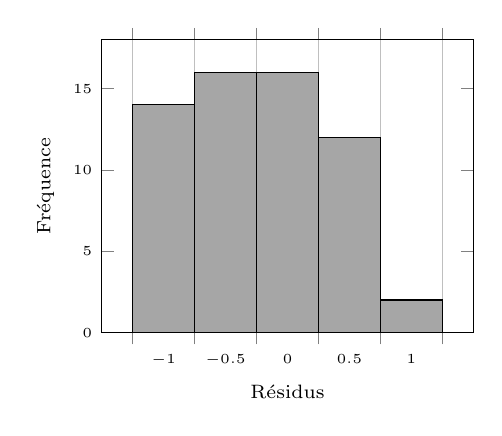
\begin{tikzpicture}
\begin{axis}[width=6.3cm, height=5.3cm, ybar interval, ymin=0, ymax=18,
  xtick={-1,-0.5,...,1.5}, xlabel={Résidus}, ylabel={Fréquence},
  tick label style={font=\tiny}, label style={font=\scriptsize}]
  \addplot[fill=black!35, draw=black] coordinates
    {(-1,14) (-0.5,16) (0,16) (0.5,12) (1,2) (1.5,0)};
\end{axis}
\end{tikzpicture}
\hspace{3mm}
\begin{tikzpicture}
\begin{axis}[width=6.3cm, height=5.3cm, xlabel={Quantiles théoriques},
  ylabel={Résidus ordonnés}, title={Diagramme quantile-quantile normal},
  tick label style={font=\tiny}, label style={font=\scriptsize},
  title style={font=\scriptsize}, grid=major, grid style={black!10}]
  \addplot[burntorange, thick, domain=-2.5:2.5] {0.568*x};
  \addplot[only marks, mark=o, mark size=1.2pt] coordinates {
  (-2.394,-0.976) (-1.960,-0.971) (-1.732,-0.832) (-1.569,-0.809) (-1.440,-0.781) (-1.331,-0.751)
  (-1.235,-0.742) (-1.150,-0.687) (-1.073,-0.687) (-1.001,-0.686) (-0.935,-0.557) (-0.872,-0.540)
  (-0.812,-0.539) (-0.755,-0.529) (-0.701,-0.500) (-0.648,-0.436) (-0.598,-0.390) (-0.549,-0.359)
  (-0.501,-0.359) (-0.454,-0.357) (-0.408,-0.319) (-0.363,-0.272) (-0.319,-0.236) (-0.275,-0.231)
  (-0.232,-0.200) (-0.189,-0.177) (-0.147,-0.161) (-0.105,-0.102) (-0.063,-0.076) (-0.021,-0.030)
  (0.021,0.038) (0.063,0.049) (0.105,0.064) (0.147,0.069) (0.189,0.108) (0.232,0.170)
  (0.275,0.178) (0.319,0.239) (0.363,0.254) (0.408,0.270) (0.454,0.284) (0.501,0.288)
  (0.549,0.291) (0.598,0.393) (0.648,0.404) (0.701,0.473) (0.755,0.503) (0.812,0.553)
  (0.872,0.590) (0.935,0.608) (1.001,0.621) (1.073,0.680) (1.150,0.689) (1.235,0.693)
  (1.331,0.809) (1.440,0.938) (1.569,0.951) (1.732,0.980) (1.960,1.001) (2.394,1.114)};
\end{axis}
\end{tikzpicture}
\end{center}

\end{frame}

\begin{frame}[t]{Homogénéité de la variance}

Diagramme de dispersion des résidus en fonction des valeurs prédites:

\begin{center}
\begin{tikzpicture}
\begin{axis}[width=9.5cm, height=5.6cm, xlabel={Valeurs prédites}, ylabel={Résidus},
  tick label style={font=\scriptsize}, label style={font=\small},
  grid=major, grid style={black!10}, ymin=-1.3, ymax=1.3]
  \addplot[black!50, dashed, domain=2.5:5] {0};
  \addplot[only marks, mark=o, mark size=1.5pt]
    table[x expr={\bzero+\bun*\thisrow{x}},
          y expr={\thisrow{y}-(\bzero+\bun*\thisrow{x})}] {\tomates};
\end{axis}
\end{tikzpicture}
\end{center}

\end{frame}

\begin{frame}[t]{Réponses}

\scriptsize
\begin{itemize}\itemsep1mm
  \item \textbf{IC pour la moyenne à 6,5\,h:} $\hat y=1{,}3724+0{,}4313(6{,}5)=4{,}18$;
  $4{,}18\pm2{,}00\sqrt{0{,}3228\,(1/60+1/175)}=4{,}18\pm0{,}17$, soit $[4{,}01;\ 4{,}35]$ kg.
  \item \textbf{Précision optimale} en $x^*=\overline{x}=5{,}5$\,h (le terme
  $(x^*-\overline{x})^2$ s'annule).
  \item \textbf{Prédiction:} même estimation ponctuelle (4,18 kg), mais erreur-type plus
  grande; IP à 95\,\%: $4{,}18\pm2{,}00\sqrt{0{,}3228\,(1+1/60+1/175)}=4{,}18\pm1{,}15$,
  soit $[3{,}03;\ 5{,}33]$ kg.
  \item \textbf{$R^2$}$\,=SSR/SST=32{,}547/51{,}268=0{,}635$: 63,5\,\% de la variabilité
  de la production est expliquée par l'ensoleillement. $R^2=0$ si $b_1=0$ ($SSR=0$);
  $R^2=1$ si tous les points sont sur la droite ($SSE=0$).
  \item \textbf{$r$:} $r>0$ si $b_1>0$, $r<0$ si $b_1<0$. Exemple:
  $r=+\sqrt{0{,}635}=0{,}797$.
  \item \textbf{Résidus:} donnée 51: $\hat y=4{,}82$, $\hat\varepsilon=-0{,}74$.
  \item \textbf{Postulats:} histogramme et QQ-plot compatibles avec la normalité;
  dispersion des résidus à peu près constante selon les valeurs prédites.
\end{itemize}

\end{frame}

\end{document}
